\documentclass[12pt,a4paper,UTF8]{article}
\usepackage{ctex} % Chinese support
\usepackage{graphicx} % Insert images
\usepackage{subfigure}
\usepackage{float}
\usepackage{listings} % Print source code
\usepackage{color} % Color support
\usepackage{booktabs} % Professional table support
\usepackage{pdflscape} % Landscape pages support in PDF
\usepackage{hyperref} % Hypertext links support for cross-referencing
\usepackage{amsmath,mathtools}
\usepackage{ulem} % strikethrough

% Customize hyperref format (it's set to no special format here)
\hypersetup{hidelinks}

% Declare directories to search for graphics files for graphicx
\graphicspath{{figures/}}

% Define source code style for listings
\lstdefinestyle{verilog-style}{
	language=Verilog,
	basicstyle=\ttfamily\footnotesize,
	keywordstyle=\bfseries\color[rgb]{0, 0, 1},
	identifierstyle=\color[rgb]{0.5, 0.3, 0.1},
	stringstyle=\color[rgb]{0.6, 0.1, 0.1},
	commentstyle=\itshape\color[rgb]{0.05, 0.5, 0.05},
	backgroundcolor=\color[gray]{0.95},
	numbers=left,
	numbersep=5pt,
	numberstyle=\color[gray]{0.6},
	breaklines=true
}

\lstdefinestyle{cpp-style}{
  language=C++,
  basicstyle=\ttfamily\footnotesize,
  keywordstyle=\bfseries\color[rgb]{0, 0, 1},
  identifierstyle=\color[rgb]{0.5, 0.3, 0.1},
  stringstyle=\color[rgb]{0.6, 0.1, 0.1},
  commentstyle=\itshape\color[rgb]{0.05, 0.5, 0.05},
  backgroundcolor=\color[gray]{0.95},
  numbers=left,
  numbersep=5pt,
  numberstyle=\color[gray]{0.6},
  breaklines=true
}

\newcommand{\reporttitle}[2]{
  \LARGE\textsf{#1}\quad\underline{\makebox[12em]{#2}}
}

\newcommand{\reportinfo}[2]{
  \large\makebox[4em]{\textsf{#1}}\quad\underline{\makebox[18em]{#2}}
}

\begin{document}
\begin{titlepage}
  \centering
  \vspace*{\fill}
  {\Huge\textsf{数字电路与数字系统实验}} \\ [100pt]
  \reportinfo{实验名称}{exp09 VGA接口控制器实现} \\ [10pt]
  \reportinfo{院系}{计算机科学与技术系} \\ [10pt]
  \reportinfo{学生姓名}{} \\ [10pt]
  \reportinfo{学号}{} \\ [10pt]
  \reportinfo{班级}{数字电路与数字系统实验1班} \\ [10pt]
  \reportinfo{邮箱}{} \\ [10pt]
  \reportinfo{实验时间}{2020 年 11 月 1 日} \\ [10pt]
  \vspace*{\fill}
\end{titlepage}
\tableofcontents
\newpage

\section{实验目的}
\begin{itemize}
  \item 学习VGA接口的原理
  \item 学习VGA接口控制器的设计方法
\end{itemize}


\section{实验原理}
图像的显示是以像素(点)为单位。从屏幕的左上角开始,一行一行
扫描每一个像素,然后输出到显示屏上。扫描一遍得到的就是一帧图像。
在标准的640$\times$480的VGA上有效地显示一行信号需要
96+48+640+16=800个像素点的时间,有效显示一帧图像需要
2+33+480+10=525个行时间。VGA\linebreak[4]
显示器一般的刷新频率是60HZ。
因此每秒扫描60帧共需要约25M个像素点的时间。


\section{实验环境/器材}
\begin{itemize}
  \item Quartus编辑器和DE10-Standard开发平台
  \item FPGA开发板
  \item 带有VGA接口的显示器
\end{itemize}

\section{程序代码+实验过程}

我把显示静态图片的两个模块放在一个工程里,用\mbox{KEY[1]}
进行控制。松开时显示图``不同颜色的条纹'',按下时显示实验提供
的mif格式的图片。\mbox{KEY[0]}是两个模块共用的reset按钮。

\subsection{实验9.3.1 显示不同颜色条纹}
实验题目里已经封装好了两个模块,我们直接调用即可。
需要我们自己实现的功能是控制每个像素点输出的颜色
(变量\mbox{vga\_data})。
\begin{lstlisting}[style=verilog-style]
always @ (posedge clk) begin
if (v_addr < 80 
   || (v_addr >= 240 && v_addr < 320)
   ) vga_data <= 12'hF00;
else if ((v_addr >= 80 && v_addr < 160)
   || (v_addr >= 320 && v_addr < 400)
   ) vga_data <= 12'h0F0;
else if ((v_addr >= 160 && v_addr < 240)
   || (v_addr >= 400 && v_addr < 480)
   ) vga_data <= 12'h00F;
else vga_data <= 12'h0;
end 
\end{lstlisting}

效果如下:
\begin{figure}[H]
  \centering
  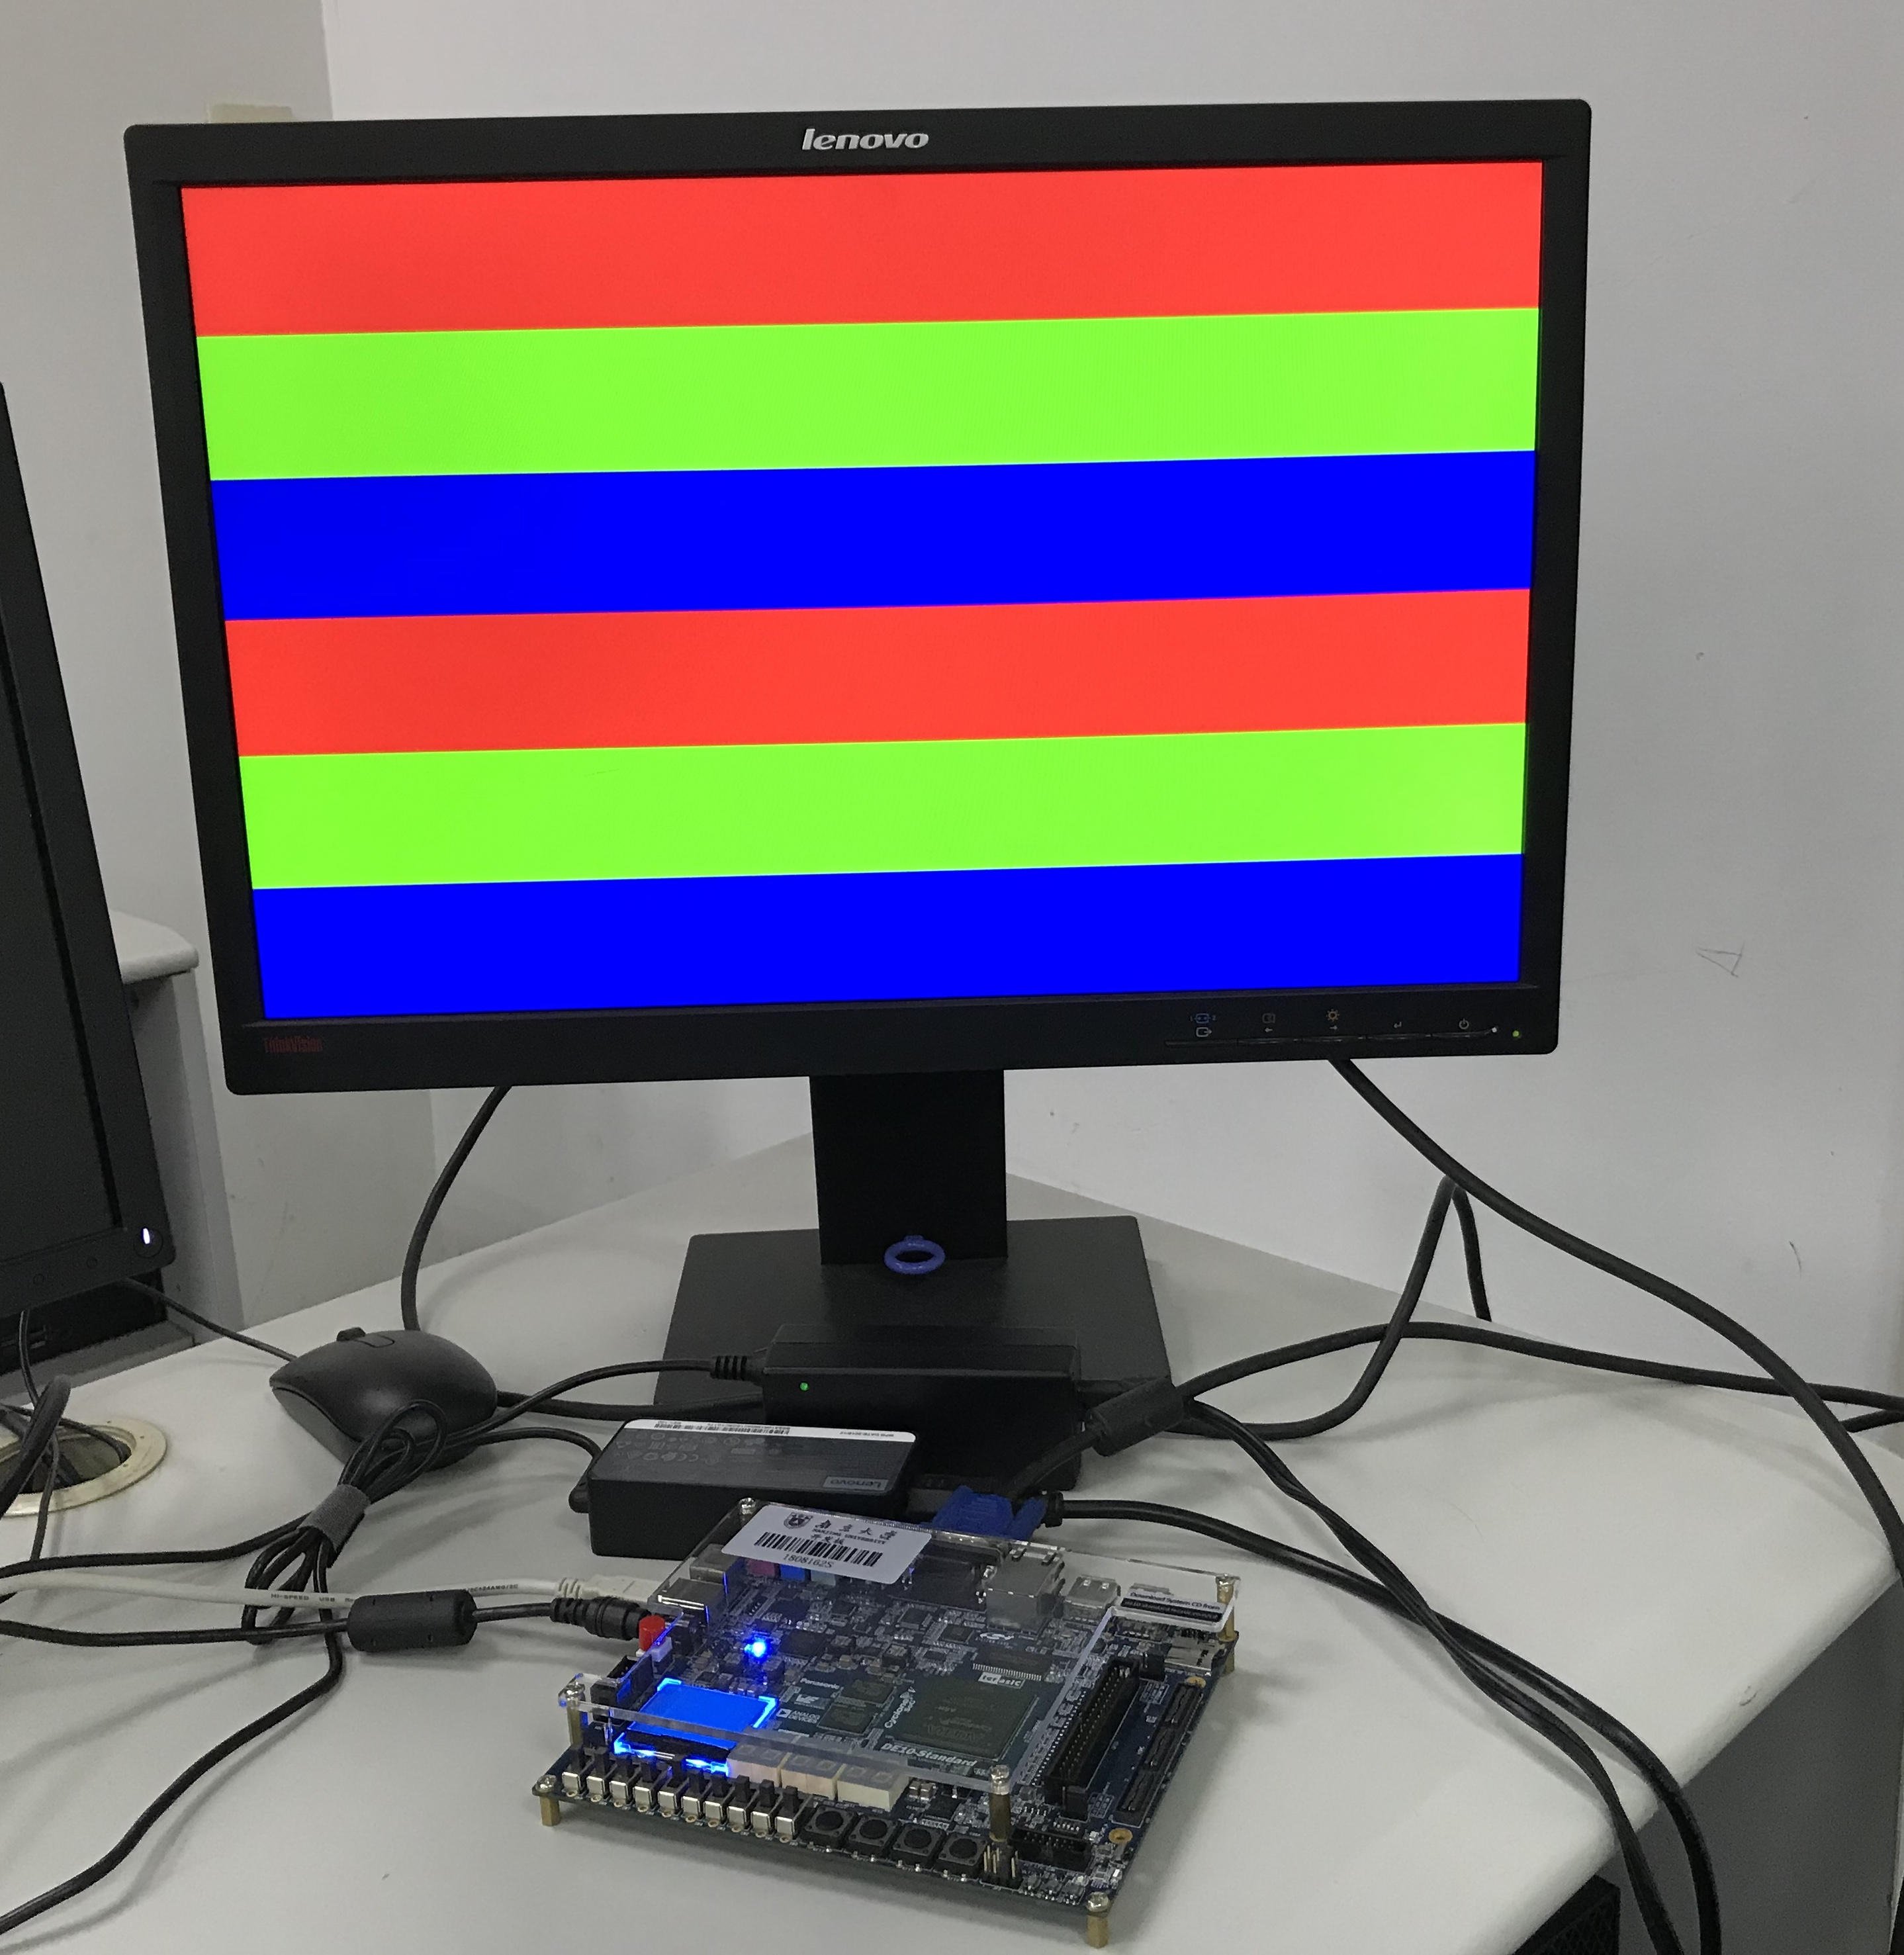
\includegraphics[width=0.8\textwidth]{img1.JPG}
  \caption{显示画面}
  \label{img1}
\end{figure}


\subsection{实验9.3.2 显示静态图片}
这个实验更简单了。我们只需要用实验提供的.mif文件初始化
一下存储器,然后按坐标输出相应颜色即可:
\begin{lstlisting}[style=verilog-style]
always @ (posedge clk) begin
    vga_data <= ram[{h_addr[9:0], v_addr[8:0]}];
end
\end{lstlisting}

效果如下:
\begin{figure}[H]
  \centering
  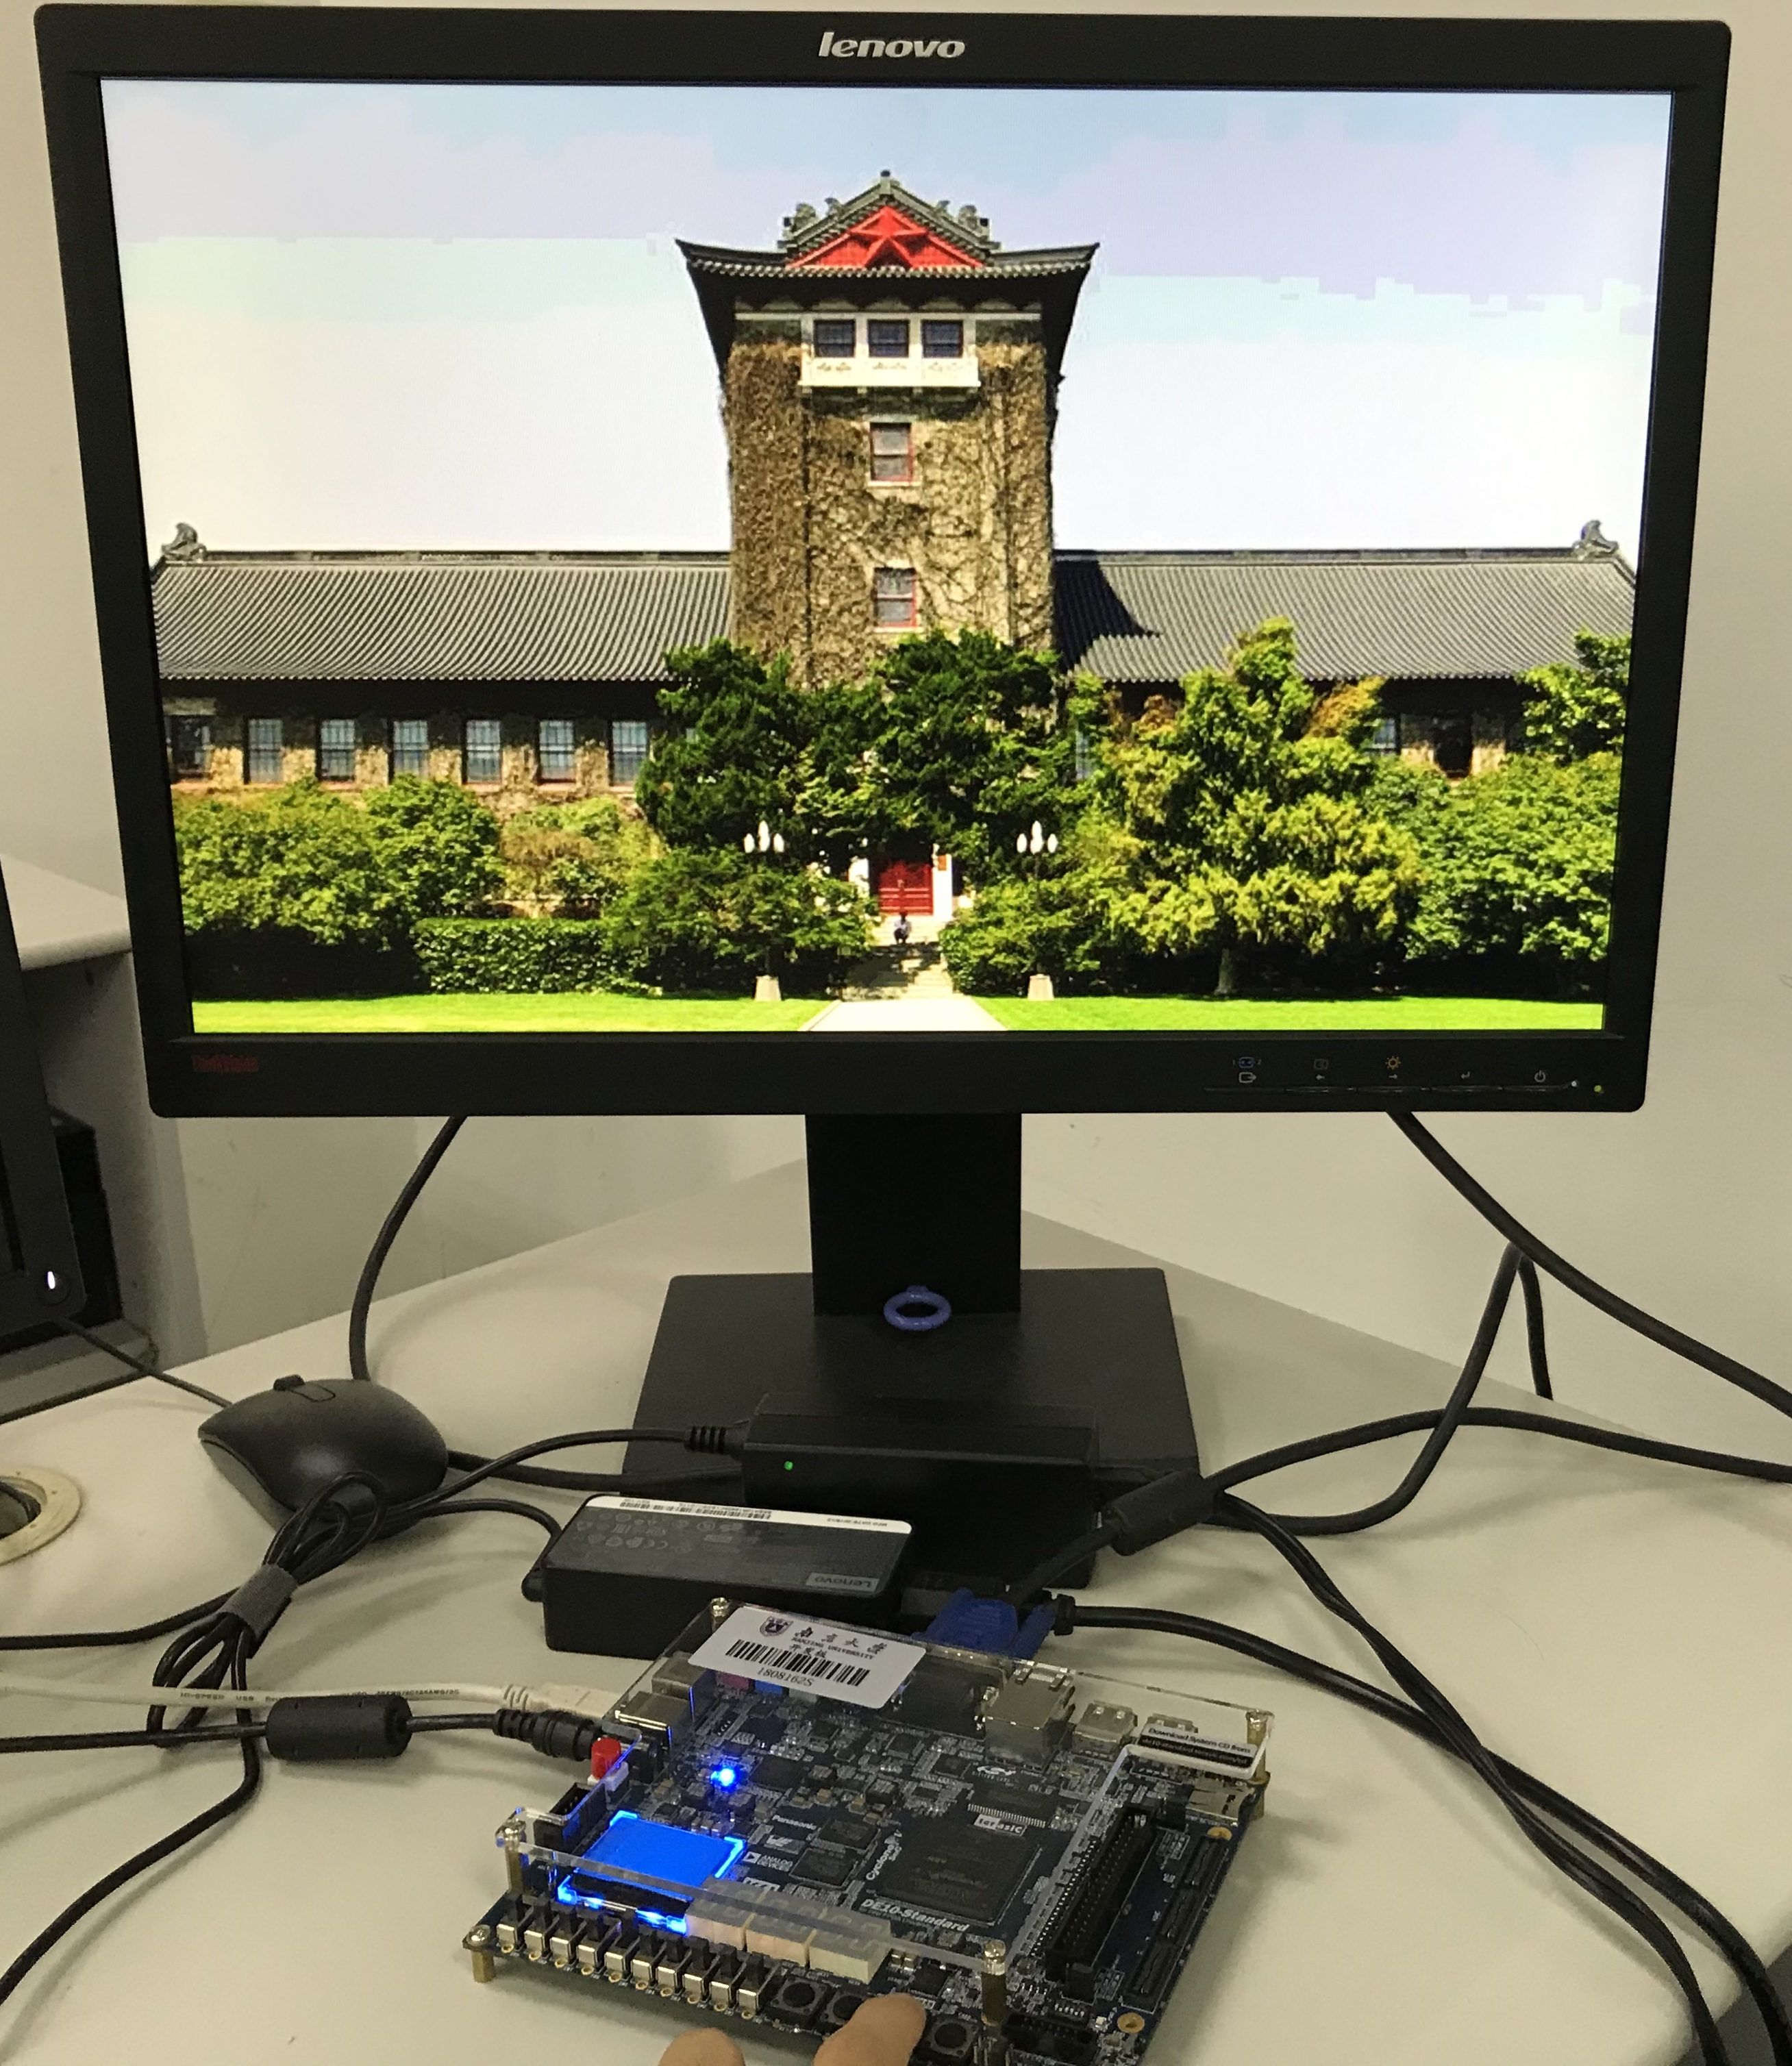
\includegraphics[width=0.8\textwidth]{img2.JPG}
  \caption{显示画面}
  \label{img2}
\end{figure}

另外还可以自己定义一些奇奇怪怪的图片:
\begin{figure}[H]
  \centering
  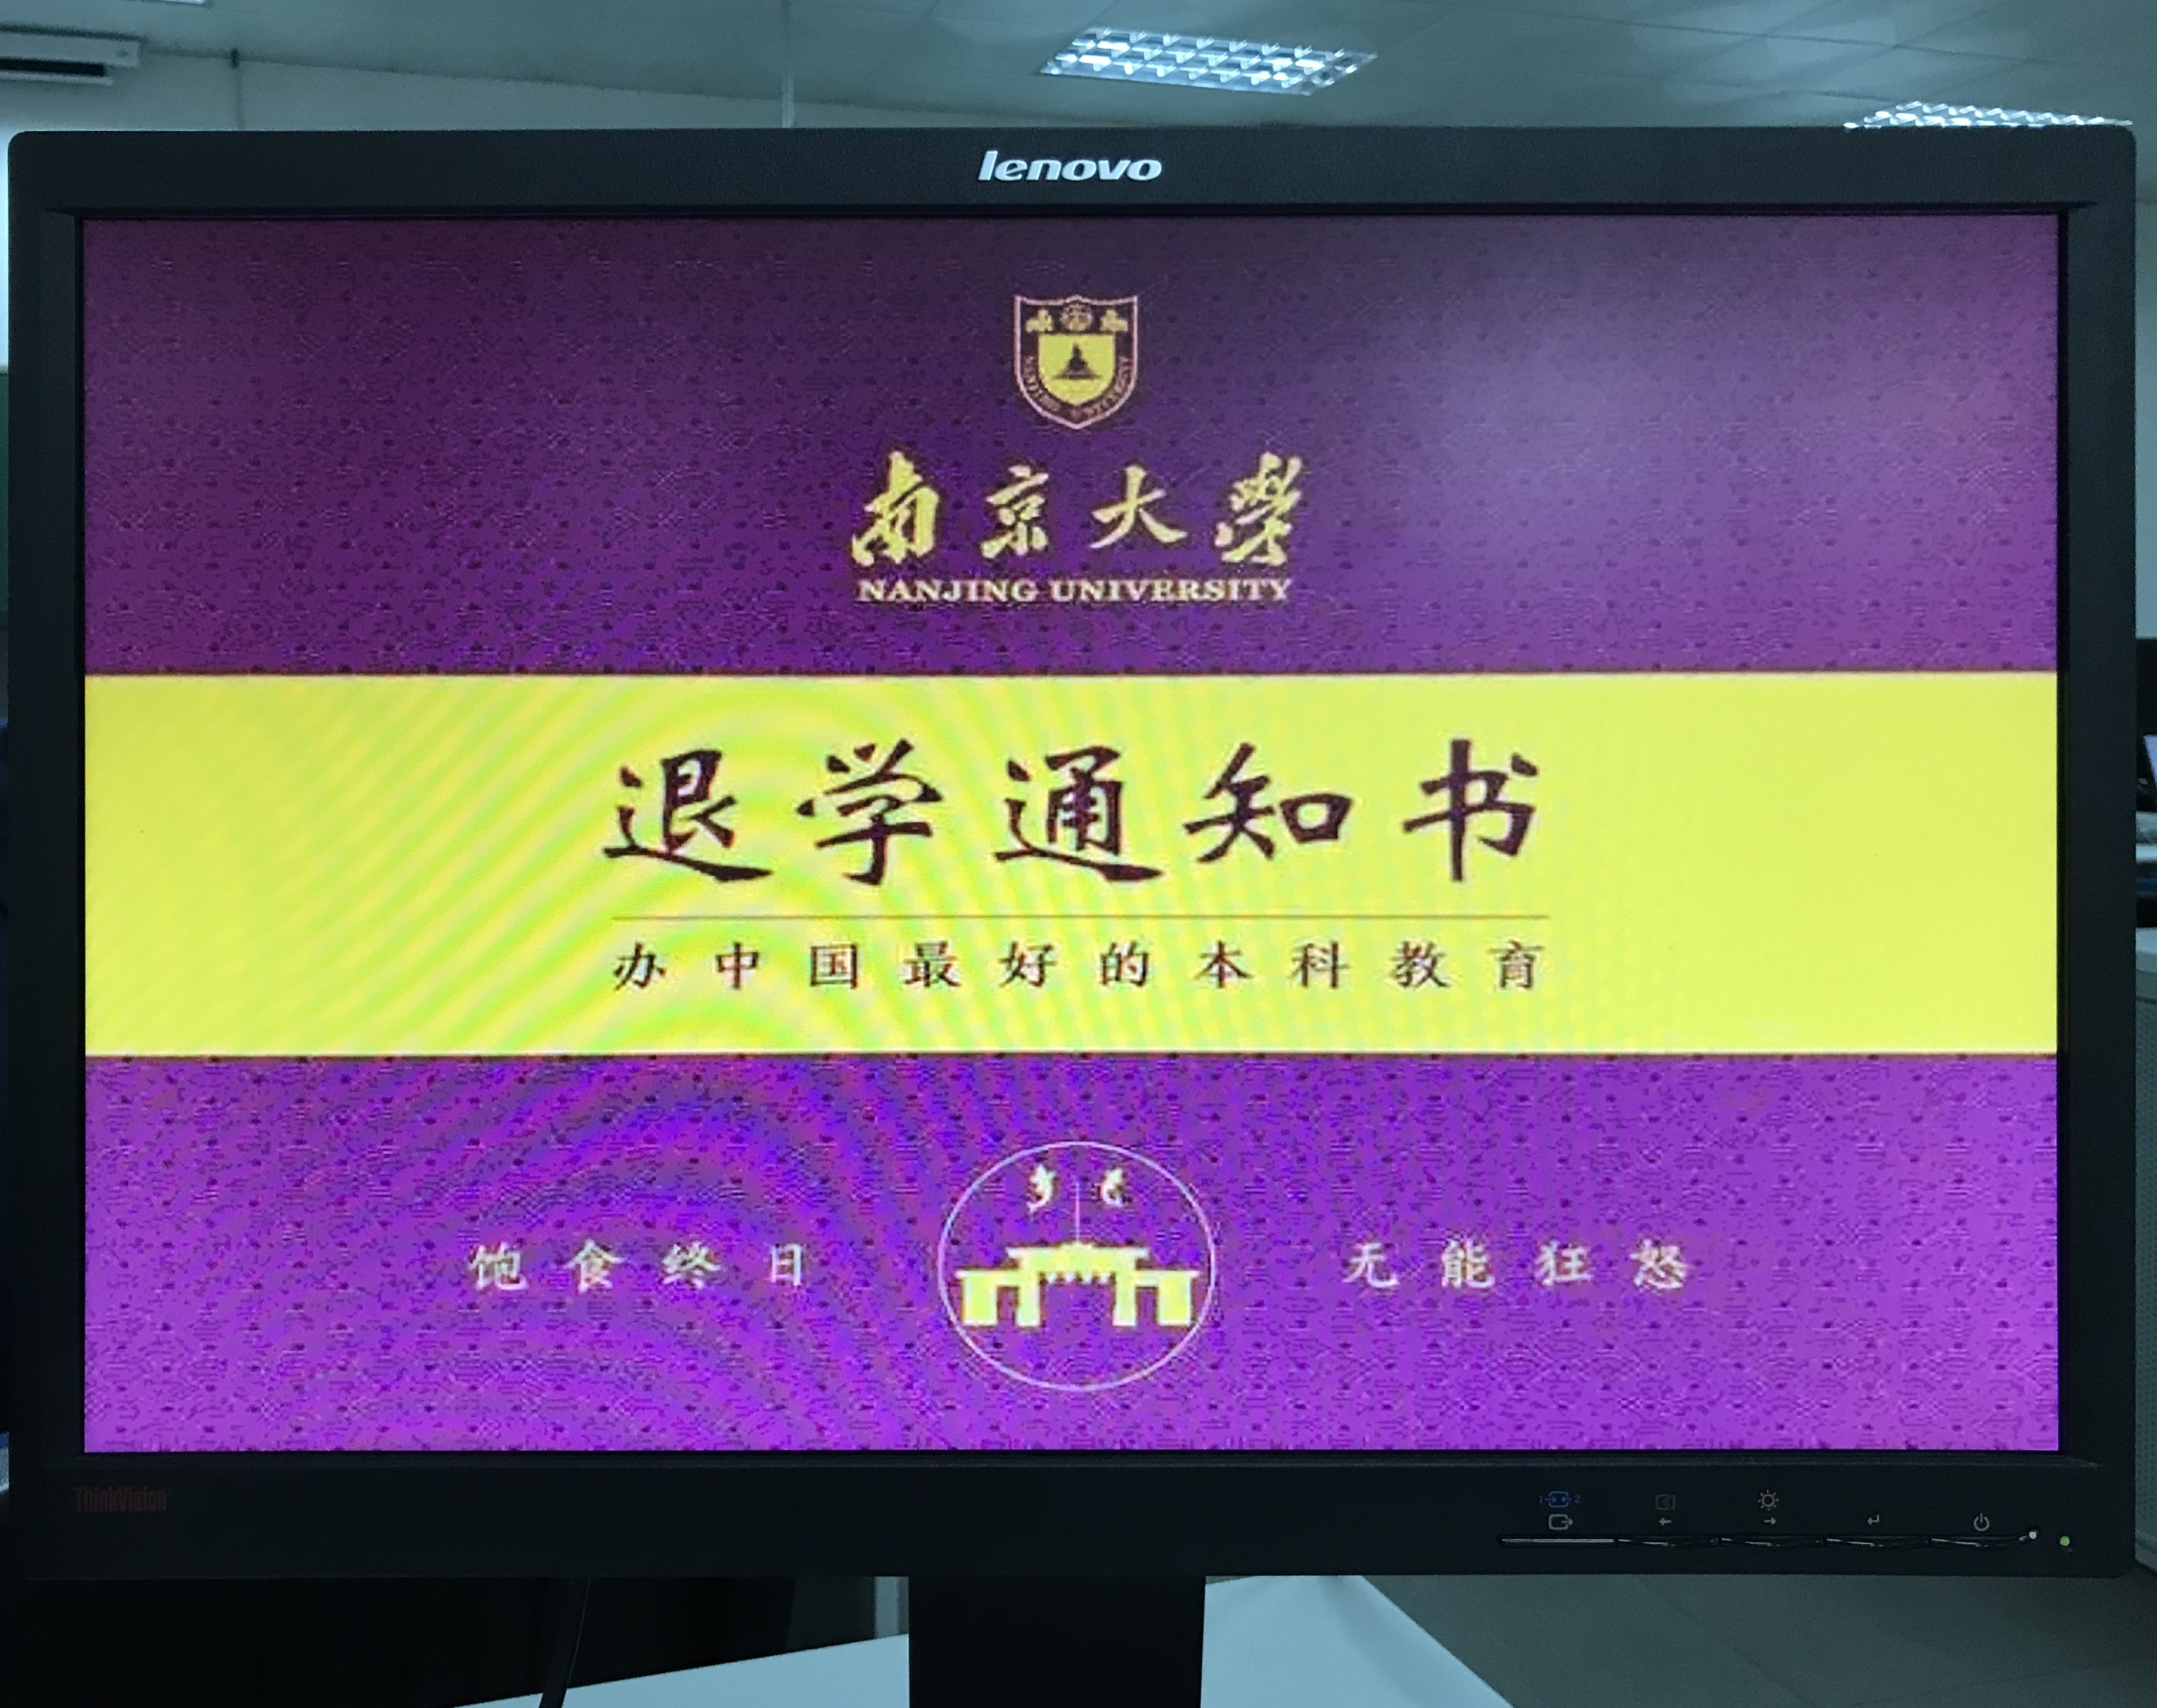
\includegraphics[width=0.8\textwidth]{img3.JPG}
  \caption{自定义图片}
  \label{img3}
\end{figure}

\subsection{实验9.3.2 拓展:在屏幕内移动的图片}
拓展功能要求:显示一张自定义的图片,使其在屏幕上按特定速度移动,
当图片边界触及屏幕边界时按弹性碰撞方式改变运动方向。

我先用c++写一个64$\times$64的红色方块作为我的自定义图片:
\begin{lstlisting}[style=cpp-style]
  #include <iostream>
  #include <fstream>
  #include <iomanip>
  
  const char* MIF_FILE = "red.mif";
  const int MIF_SIZE = 4096;
  
  int main() {
    std::ofstream red_pic(MIF_FILE);
    if (!red_pic.is_open()) {
      std::cout << "open error\n";
      return -1;
    }
  
    red_pic << "WIDTH = 12;\nDEPTH = " << MIF_SIZE << ";"
            << "\nADDRESS_RADIX = HEX;\nDATA_RADIX = HEX;\n\n"
            << "CONTENT BEGIN\n";
  
    for (int i = 0; i < MIF_SIZE; ++i) {
      red_pic << std::setw(8) << std::setfill('0') << std::hex
              << i << ": F00;\n";
    }
    red_pic << "END;";
    red_pic.close();
  
    return 0;
  }
\end{lstlisting}

实验提供了一份参考代码,修改一下就能为我所用了。二话不说,
先把parameter参数\mbox{logo\_length}和\mbox{logo\_hight}
改成64,再把\mbox{rom\_addr}改成12位的形式。

然后来解读一下实验提供的代码(已修改):

首先是调用一些模块,其中只有\mbox{logo\_rom}模块需要自己
编写一下。这个模块也很简单,只需要用自定义的.mif文件初始化
一个存储器,然后根据传入的参数寻址输出存储器中相应颜色即可。
用assign即可解决问题,可以不用时钟信号。

接着需要给变量\mbox{logo\_area}赋值。当\mbox{logo\_area}
为1时,说明此时扫描的像素位于自定义图片的区域内,需要输出自定义
图片对应像素的颜色。\linebreak[4]
\mbox{logo\_area}为0时,明此时扫描的像素
不在自定义图片的区域内,输出黑色即可。always块如下:
\begin{lstlisting}[style=verilog-style]
assign logo_area = ((v_cnt >= logo_y) 
    & (v_cnt <= logo_y + logo_hight - 1) 
    & (h_cnt >= logo_x) 
    & (h_cnt <= logo_x + logo_length - 1)) 
  ? 1'b1 : 1'b0;
always @(posedge pclk) begin: logo_display
  if (rst == 1'b1)
     vga_data <= 12'b000000000000;
  else begin
     if (valid == 1'b1) begin
        if (logo_area == 1'b1) begin
           rom_addr <= rom_addr + 12'b01;
           vga_data <= douta;
        end else begin
           rom_addr <= rom_addr;
           vga_data <= 12'b000000000000;
        end
     end else begin
        vga_data <= 12'b111111111111;
        if (v_cnt == 1)
           rom_addr <= 12'b0;
     end
  end
end
\end{lstlisting}

我们需要控制图片的移动速度。当\mbox{speed\_ctrl}为1时,
图片移动一格。与之相关的代码如下:
\begin{lstlisting}[style=verilog-style]  
always @(posedge pclk) begin: speed_control
  if (rst == 1'b1)
     speed_cnt <= 8'h00;
  else begin
     if ((v_cnt[5] == 1'b1) & (h_cnt == 1))
        speed_cnt <= speed_cnt + 8'h01;
  end
end

debounce u3(
  .clk(pclk), 
  .sig_in(speed_cnt[5]),
  .sig_out(speed_ctrl)
  );
\end{lstlisting}

debounce模块是取参数\mbox{sig\_in}的上升沿作为返回输出:
\begin{lstlisting}[style=verilog-style]
module debounce(
  input clk,
  input  sig_in,
  output sig_out
  );
  reg q1, q2, q3;
  always @ (posedge clk)
  begin
    q1 <= sig_in;
    q2 <= q1;
    q3 <= q2;
  end
  assign sig_out = q1 & q2 & (!q3);
endmodule
\end{lstlisting}

然后只要实现图片下一步向哪个方向移动,拓展功能就大致完成了。
代码比较长所以不贴了,简单解释一下原理:
图片的移动方向只有4个,分别是左下、左上、右下、右上,
都是沿45度角运动。如果当前图片位于左下角,那么运动方向改为右上;
如果当前图片位于左上角,那么运动方向改为右下;如果当前图片位于
左侧边(除去左下角和左上角),那么运动的水平方向取反,竖直方向不变。
依次类推,四个角四条边再加上中央(不沾边且不沾角时运动方向不变),
共9种情况。分情况实现即可。

在显示器上运行效果如下:
\begin{figure}[H]
  \centering
  \subfigure{
    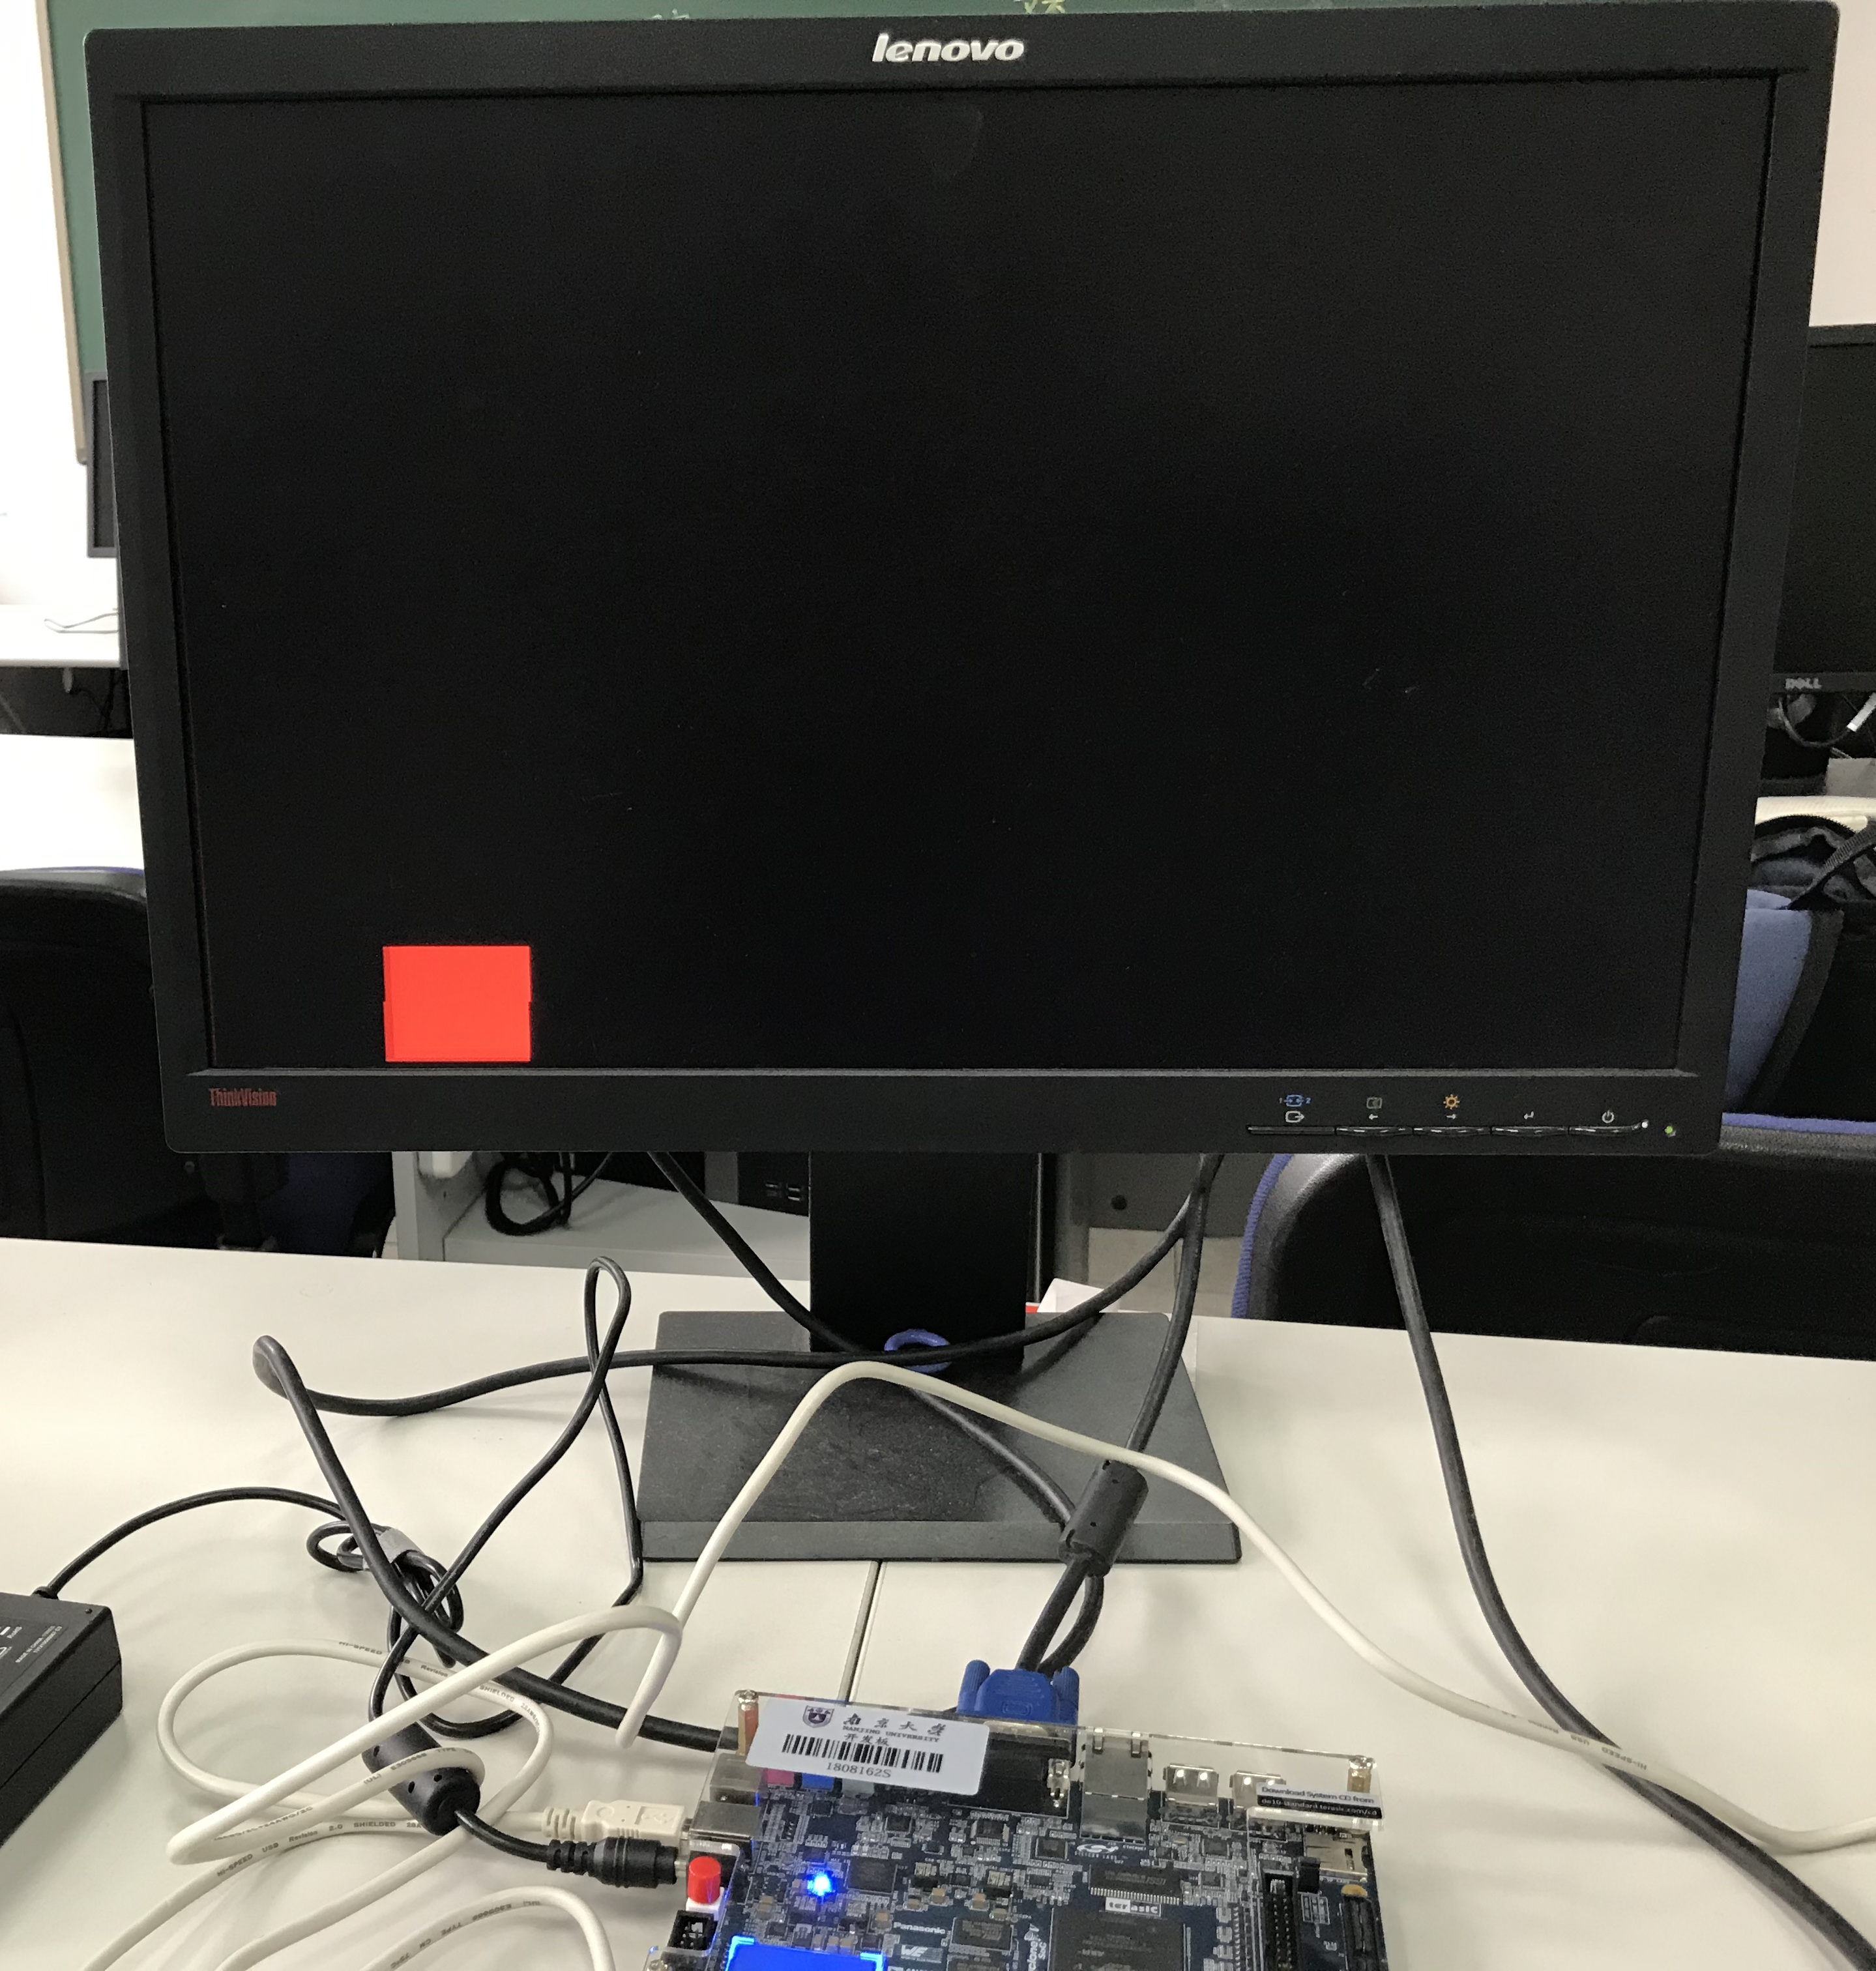
\includegraphics[width=0.45\textwidth]{img3_1.JPG}
  }
  \subfigure{
    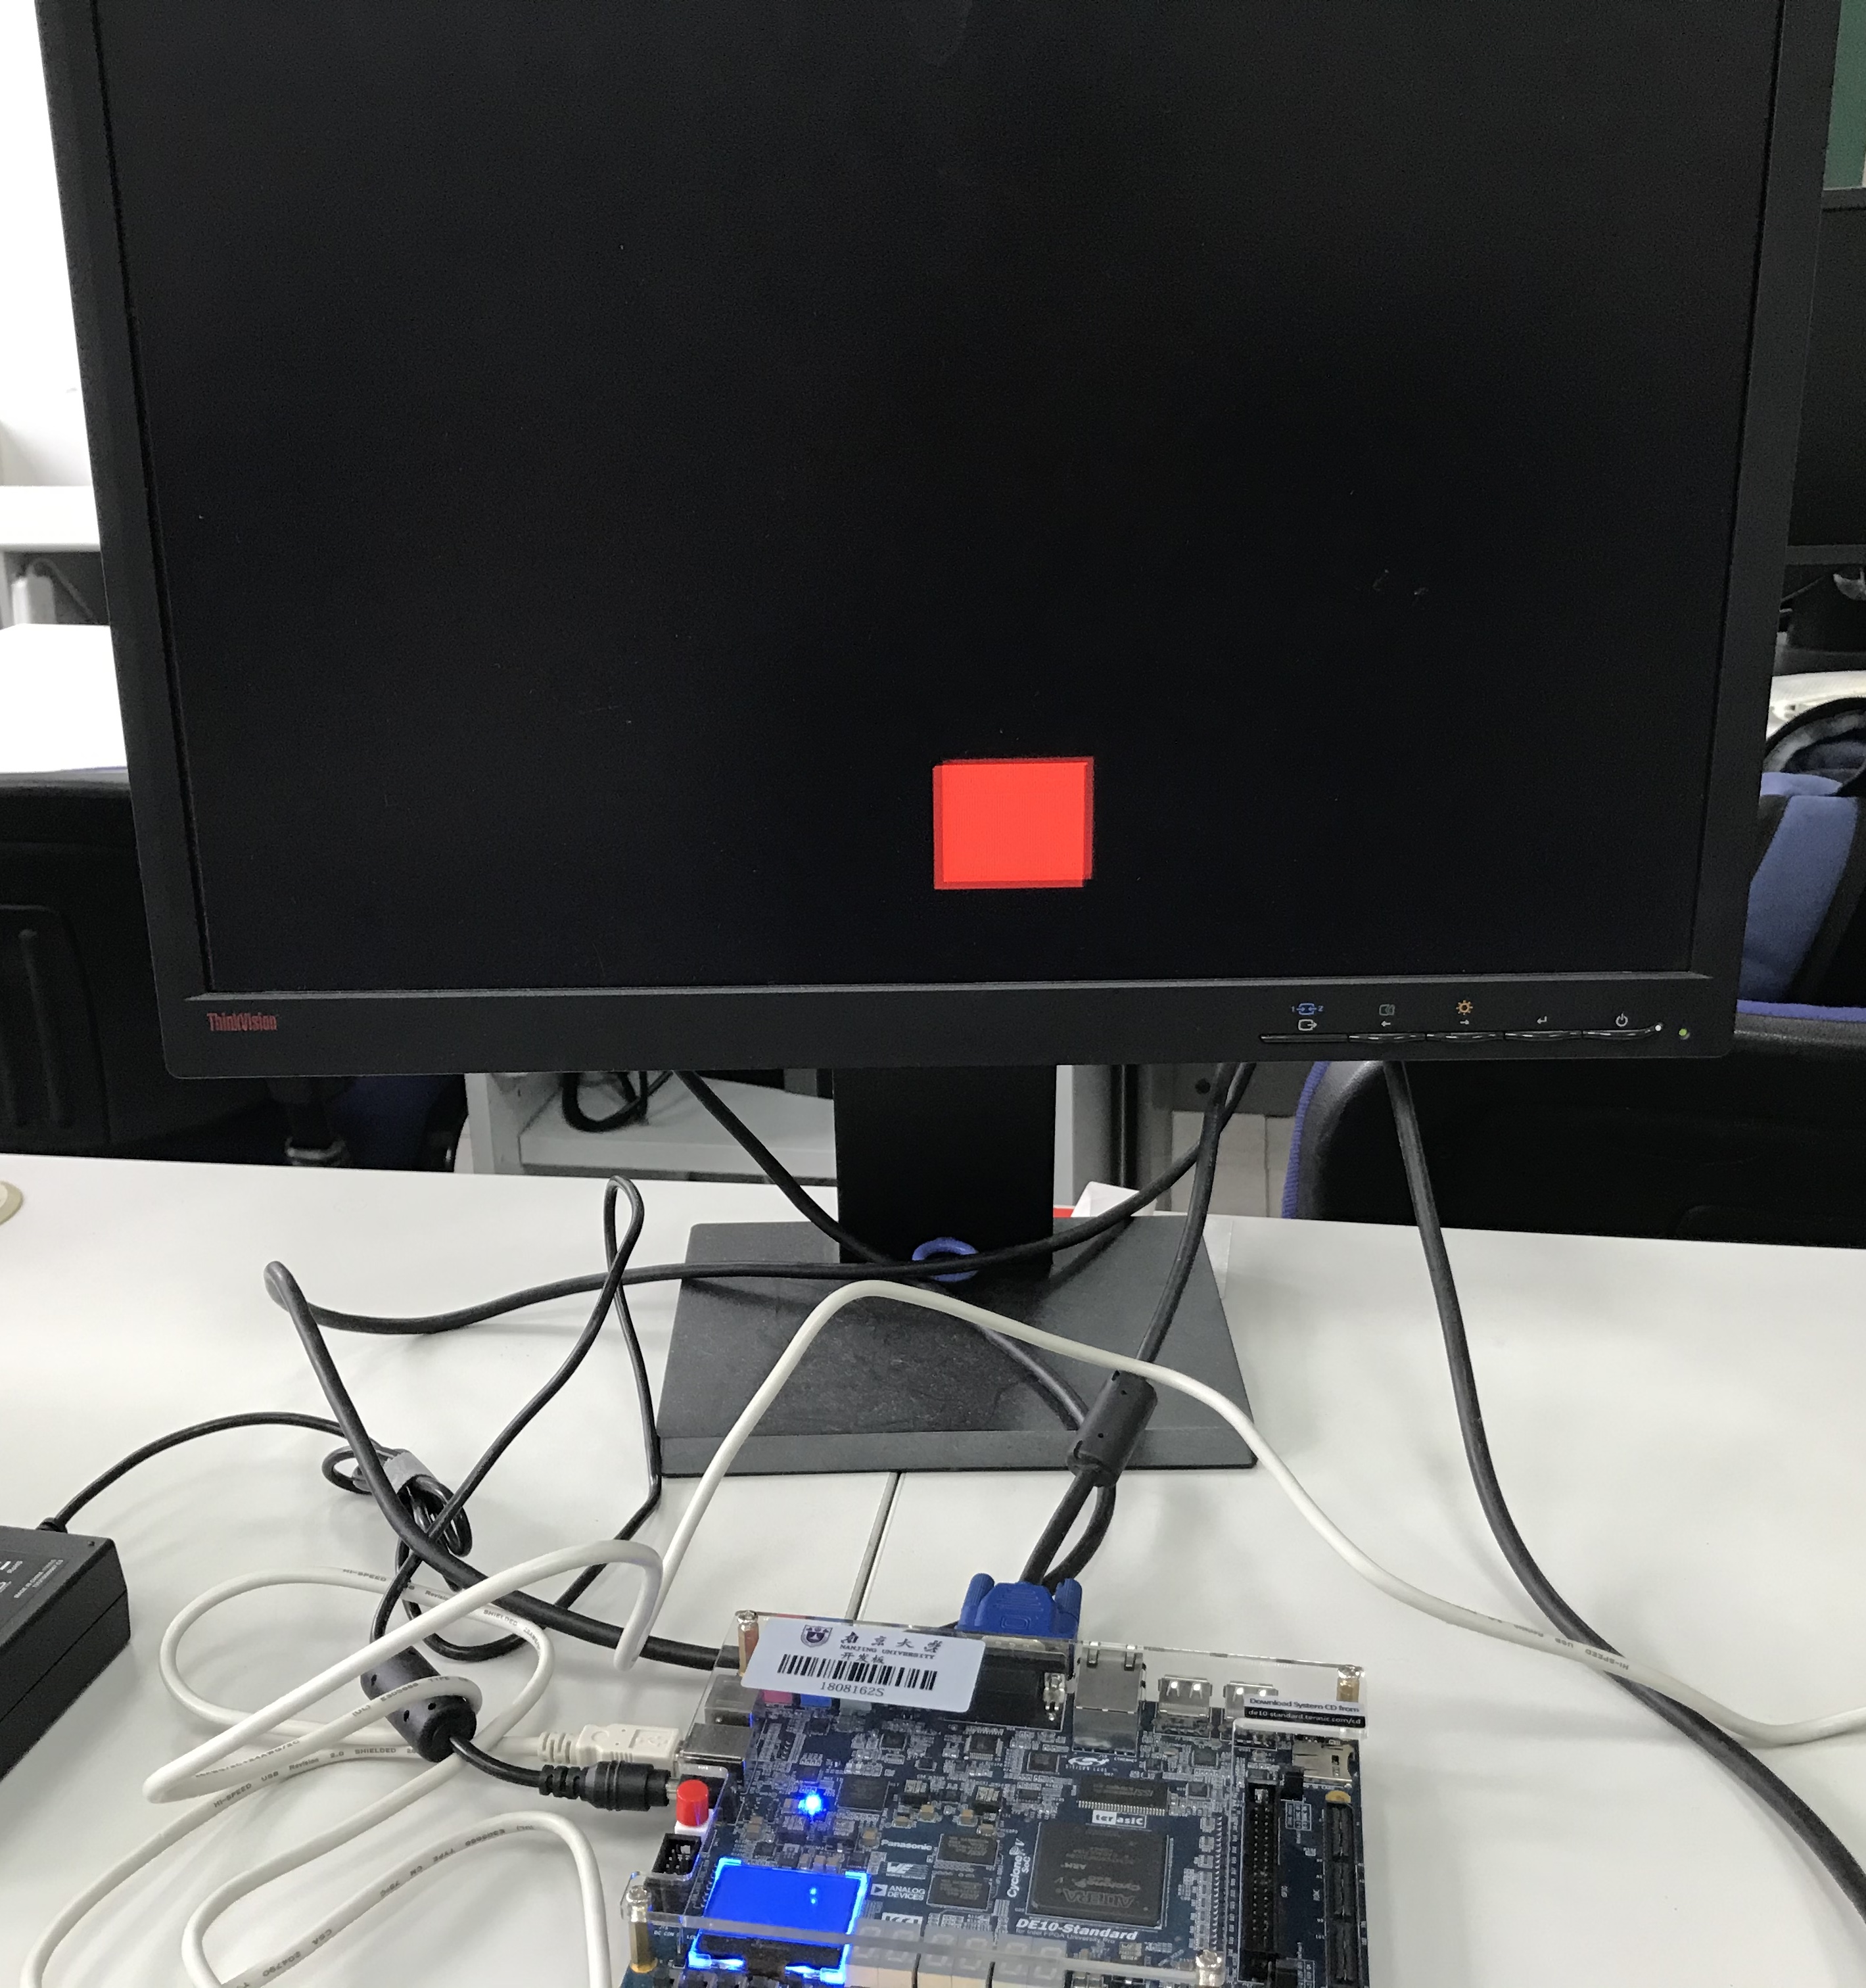
\includegraphics[width=0.45\textwidth]{img3_2.JPG}
  }
  \caption{运动中的方块}
  \label{img3}
\end{figure}


最后吐槽一下实验提供的代码:
\begin{itemize}
  \item 基础实验(两个静态图片的实验)的像素起始位置设置的是0,
        拓展实验的像素起始位置设置的是1(还好我仔细比对了一下题目
        pdf里的代码和提供的.v文件,哼哼)
  \item 在拓展实验的代码中,名为\mbox{logo\_display}的
        always块的最后一个if判断里,\mbox{v\_cnt}最小值是1
        不是0\sout{(原来老师自己也记混了嘿嘿嘿)}
  \item \sout{生怕我们看懂拓展实验提供的代码所以没加啥注释}
\end{itemize}


\section{遇到的问题及解决办法}
\begin{itemize}
  \item 如果初始化存储器的文件比较大,那么建议用.mif文件
        而不是.txt文件来初始化存储器(我用.txt跑了十几分钟
        都没编译出来,用.mif几秒钟就初始化完成了)
  \item VGA的颜色接口是8位,模块返回值是4位。一定要记得
        在顶层模块里把子模块的返回值赋给高4位,而不是直接
        把8位的接口传到子模块里。
\end{itemize}

\section{得到的启示}
\begin{itemize}
  \item 原来还可以用c++写一个图片出来(奇怪的知识增加了)
  \item \sout{觉得别人的代码不优雅就自己动手丰衣足食}
\end{itemize}

\section{意见和建议}

\sout{好久没有在数电实验题目里遇到保姆级教程了,菜鸡落泪}

\sout{希望后面的实验也能像实验9一样友好}

\end{document}